\section{Method}
\label{sec:overview}

%\begin{figure}[h]
%  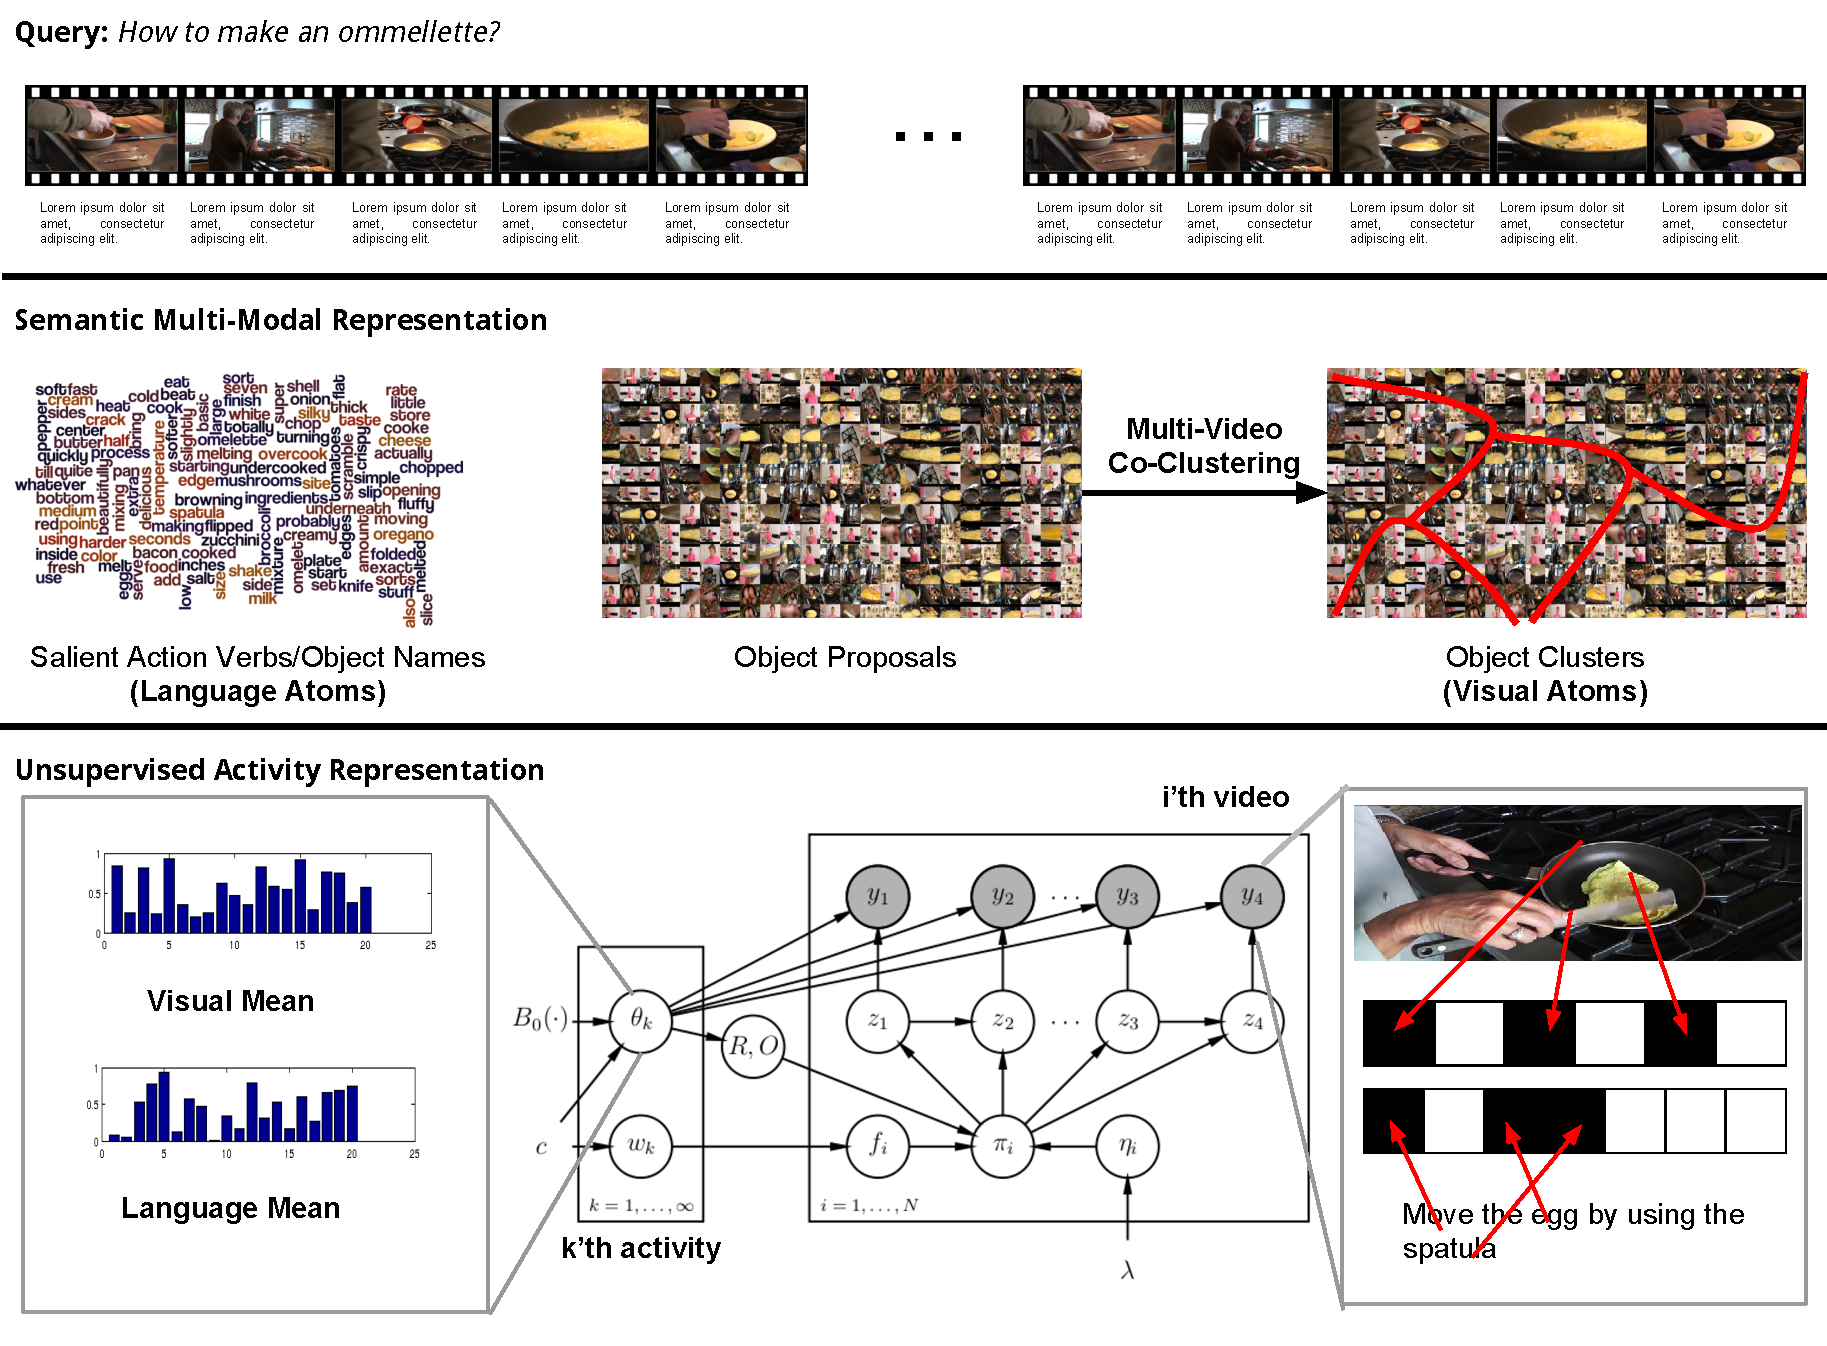
\includegraphics[width=0.5\textwidth]{algor}
%  \caption{Components of our recipe understanding method. \textbf{Query:} We query the YouTube for top 100 \emph{How To} videos and filter the outliers; \textbf{Framewise Representation:} We automatically extract object clusters and salient word in order to find multi-modal representation of each frame. \textbf{Unsupervised Activity Detection:} We jointly cluster videos in order to learn activities/steps related to the recipe.}
%\label{fig:overview}
%\end{figure}

Given a large video-collection, our algorithm starts with learning a set of visual and language atoms which are further used for representing multi-modal information. These atoms are designed in a way to correspond to the mid-level semantic concepts like actions, objects etc.. In order to learn visual atoms, we generate object proposals and cluster them into mid-level atoms. Whereas, for the language atoms we simply find the salient and frequent words in the subtitles. After learning the set of atoms, we represent the multi-modal information in each frame based based on the occurrence statistics of the learned atoms. Given a series of multi-modal frame representations, we discover set of clusters, defined via learned atoms and their temporal relations, occurring over multiple videos by using a non-parametric Bayesian method. We expect these clusters to correspond to the activity steps which construct the high level activities. Moreover, our empirical results suggest that the resulting clusters significantly correlates with the activity steps.

In Section~\ref{atoms}, we explain how do we learn the language and visual atoms. Then, we explain the multi-modal representation of the frames in Section~\ref{representation}. And, finally we explain how do we discover activity steps in Section~\ref{learning}.


%In this section, we explain the high-level components of our method which we visualize in Figure~\ref{fig:overview}. Our proposed method consists of three major components; \textbf{(1) Online query and filtering:} Our system starts with querying the YouTube with an \emph{How to} question, and records the top 100 resulting videos. In order to detect the similarity of the videos quickly, we also process the text descriptions and eliminate outliers. \textbf{(2) Frame-wise multi-modal representation:} In order to semantically represent the spatio-temporal information in the videos, we process both the visual and language content of each video. We extract the region proposals and jointly cluster them to detect semantic visual objects. We also detect the salient words of the subtitles. Finally, we epresent the each frame in terms of the resulting objects and the salient words. \textbf{(3) Unsupervised joint clustering:} After describing the each frame by using both language and visual cues, we apply 

